 
\section{Our focus and plan}

% % % TODO % % % %
%from rules: Innovative technology (if any) TODO describe usage of STRANDS
%from rules: Reusability of the system or parts thereof - see STRANDS
This section summarises our intentions for our system this year. We would like to aim for high re-usability of code in our robotic system and to demonstrate that the current state of the art in AI algorithms mixed with our extensions can be successfully used to produce a robust, effective and complete robotic system with domestic applications.  

%\subsection{Catering for Granny Annie’s Comfort}
%
%A robot will receive commands from Granny Annie by natural speech. These commands may contain interaction with an intelligent flat or require the robot to bring her a specific object. 
%We have started a cooperation with a research group in this field and we hope to be able to recognise speech more robustly than using CMU Sphinx which we used last year, see Sec.~\ref{sec:speechrec}.
%
%We would like to prepare our robot so that it can perform the first part - cooperation/interaction with an intelligent flat. This subtask still contains interesting challenges, such as robust speech recognition and robot navigation in a way which is comfortable and natural for a human.  


\subsection{Getting to know my home}

In this task, a robot should recognise changes in a flat, such as open/closed doors, furniture which has been moved to another room or everyday objects which were moved. 
The robot can detect these changes autonomously or by cooperation with a human who uses speech or gestures.
After detection, the robot is asked to use this new knowledge to execute some commands, such as to bring a mug on the dining table which is now in living room.

The state machine for this task from the RoCKIn@Home 2014 is in Fig.~\ref{fig:st1}.
Our system was built on two parts - autonomous detection of doors using the laser rangefinder and cooperation with a human in order to detect where the furniture is. 
In RoCKIn@Home 2015 we extended this system and we have now fully functioning system to accomplish this task.


\begin{figure}[!htb]
\centering
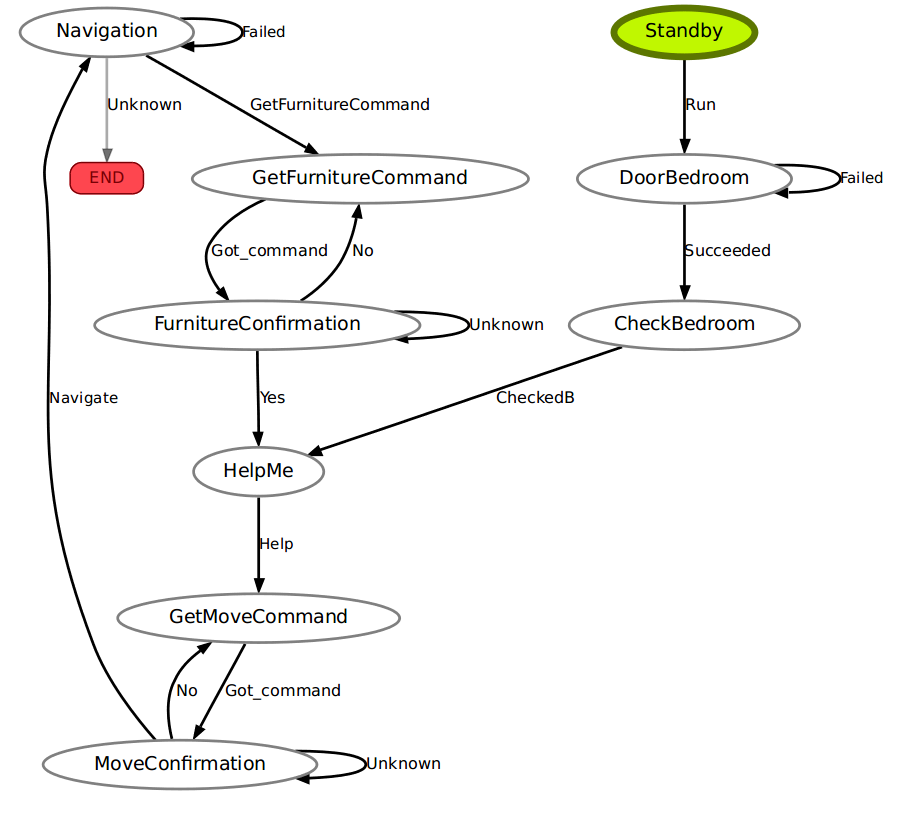
\includegraphics[width=3.in]{statemachine_t1.png}
\caption{The state machine for the task Getting to know my home}
\label{fig:st1}
\end{figure}

\subsection{Welcoming visitors}

In this task, a robot should welcome visitors, recognise them and accompany them to a specific location in Granny's flat. Several components are needed in this task: computer vision for face recognition and for uniform detection. Moreover, machine learning techniques are needed to be able to learn these two patterns in order to recognise them. A robot can also benefit from speech recognition if face/uniform recognition does not provide a certain decision. Additionally, a robot must have robust navigation in an environment in order to accompany a person to a specific place. 
Finally, human-robot interaction is needed while accompanying a person.

We successfully completed this task during the RoCKIn@Home challenges. Our system was built on several components which are mentioned in Sec.~\ref{sec:software}. 
Our core state machine is built for this task calling several components. 
We do not plan significant changes to our face recognition system, however, we will create a larger database of faces in order to improve the classification of the doctor.

Uniform recognition needs to be improved due to the following reasons.
First, uniform detection was based only on colour segmentation of the whole image. This means that if there is a significantly large object of a certain colour belonging to a uniform (white/yellow) in the background, this object will be classified as the person. We previously tried to improve this by only looking for the uniform in the region of the image below a detected face, but the face detector was not robust enough in the presence of shadows.
In addition, we plan to extend the uniform detection with a keypoint based image detector to search for the uniform logos.
Both issues were limitations last year and we are improving them.  


\subsection{Object perception} 

We have won this task in RoCKIn@Home 2015 with an approach which uses transfer learning to recognise objects using a convolutional neural network (CNN) which has been pre-trained for another task, in our case, image classification \cite{schwarz}. An RGB-D pair of images is first pre-processed as shown in Fig.~\ref{fig:object_perception}. Next, the images are processed by the CNN in order to extract a vector of image features for each RGB-D frame. This feature vector is used with a tree of classifiers and regressors to determine first the category of the object, then the object instance, and finally the pose of the object.

\begin{figure}[!htb]
\centering
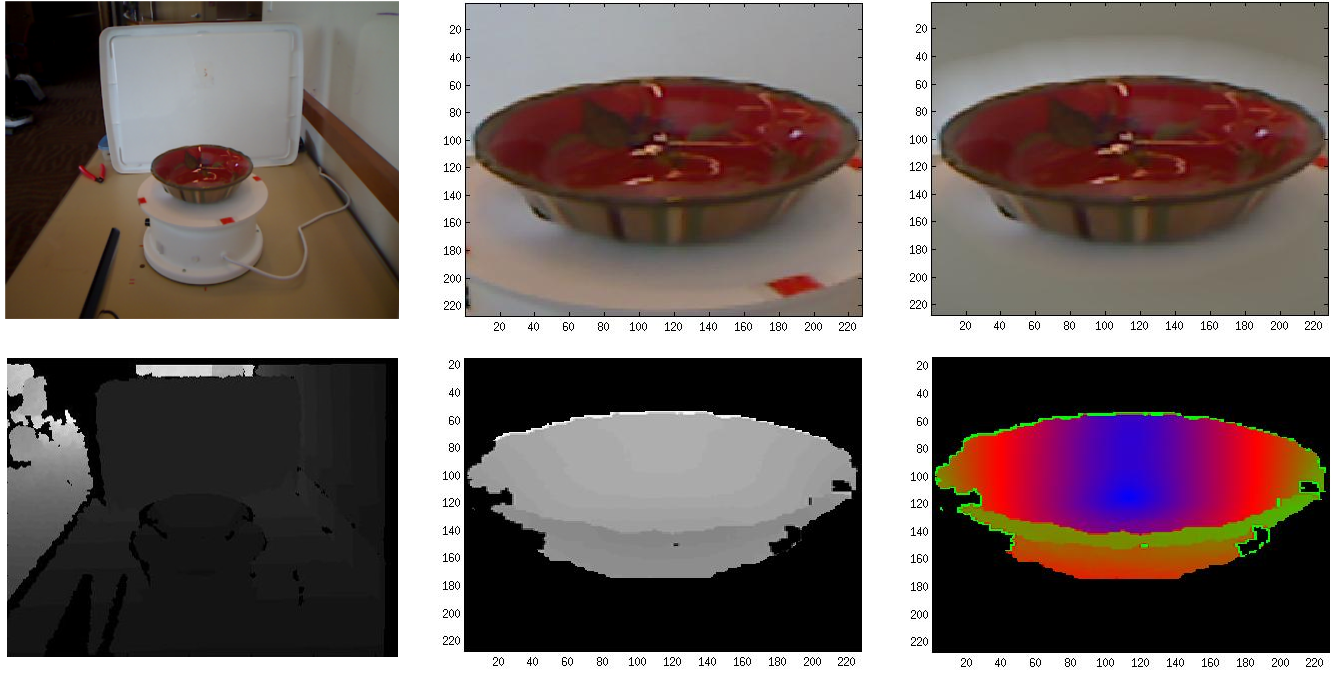
\includegraphics[width=3.in]{object_perception.png}
\caption{The image pre-processing pipeline for the described algorithm. Top: The RGB image is first cropped down to size and then a fading algorithm is used to reduce the chance of unwanted features being detected in the background of the image. Bottom: The depth image is cropped in the same way and then coloured based on the depth data. This is required because the CNN is trained to detect features in RGB images and so we want the new image to describe the depth information in RGB. Image data used from the Washington RGB-D Object Dataset \cite{lai}.}
\label{fig:object_perception}
\end{figure}

%\subsection{Navigation}

%We had robust configuration of navigation stack from ROS last year, which combined benefits from laser rangefinder and a depth camera. 
%Additionally, we have added monitored navigation to recover from failure and topological navigation in order to control behaviour of the robot in different rooms. Details are explained in Sec.~\ref{sec:software}.

%\subsection{\label{sec:speechrec}Speech understanding}

%In previous years, we used CMU Sphinx for speech recognition with no added microphone. CMU Sphinx is not good enough for this benchmark. 
%Therefore, we have started to cooperate with the speech recognition research group in our faculty in order to deploy a more sophisticated algorithm on our robot. 


\subsection{Timetable}

We intend to participate in all benchmarks except for \textit{Catering for Granny Annie's Comfort}. However, our priorities are the following.
First, we will perform the complete \textit{Getting to know my home}, \textit{Welcoming Visitors} and \textit{Object perception} benchmarks.
We expect to participate in the \textit{Visiting My Home} task benchmark and \textit{Navigation} functional benchmark. We hope to participate in the \textit{General Purpose Service Robot} and \textit{Speech Recognition}.


%\begin{figure}[!htb]
%\centering
%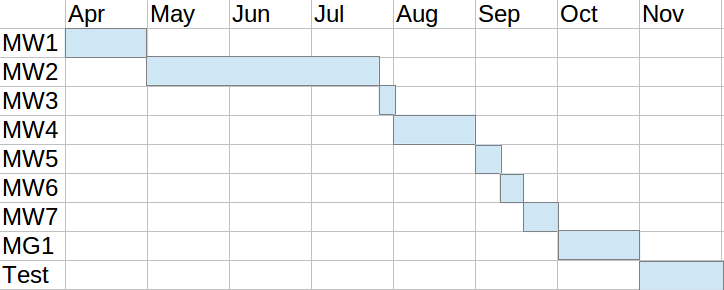
\includegraphics[width=3.in]{timetable.png}
%\caption{Timetable}
%\label{fig:plan}
%\end{figure}
